% Capítulo 3
\chapter{Arquitetura}
\label{ch:architecture}

Neste capítulo, apresenta-se o estado atual da arquitetura do sistema, na seção \ref{sec:architecture:current_components_and_architecture}, onde é descrito o funcionamento dos componentes envolvidos no processo de caminhada. Em seguida, a nova proposta é exibida, detalhando e justificando as modificações nos componentes com suas devidas implicações e impacto na arquitetura geral.

Inicialmente, a arquitetura adotada pelo time AUT-UofM é uma arquitetura distribuída, baseada no \textit{framework} \abrv[ROS -- \textit{Robot Operating System}]{ROS}. Como a robótica tenta solucionar problemas em diversas áreas da computação. Desde o controle de motores, usando programação de baixo nível, até soluções sofisticas utilizando \abrv[IA -- Inteligência artificial]{IA (Inteligência artificial)} aplicada a visão e tomada de decisões, entre outros.

Assim, o desenvolvimento de uma única ferramenta, em uma única linguagem, que solucione todos os problemas pode tornar-se inviável, já que linguagens diferentes são projetadas com intenções diferentes e problemas diferentes em mente.

\section{Componentes e arquitetura atual}
\label{sec:architecture:current_components_and_architecture}

A arquitetura do sistema pode ser abstraída em $3$ camadas: A camada de \textit{hardware}, a de software de baixo nível, e a de software.

Na camada de \textit{hardware}, a mais inferior na figura~\ref{fig:softwarearchitecture:overview}, estão contidos os componentes físicos do sistema. Uma câmera \textit{Webcam Logintech C920 Pro HD 15MP Full HD1080p} é usada para fornecer imagens para o sistema de visão. Uma \abrv[IMU -- do inglês \textit{Inertia Measurement Unit}]{IMU}, do inglês \textit{Inertia Measurement Unit}, é usada para fornecer informações para o posterior cálculo da orientação do corpo do robô em relação ao eixo de gravidade. E os motores, também chamados de atuadores, são utilizados nas juntas para os movimentos às partes do robô.

A camada de software de baixo nível é responsável pelo processamento de dados da \textit{IMU}, juntamente com a execução do \textit{walking gait}. Esta camada roda dentro da placa microcontroladora \textit{Robotis.Co OpenCM9.04}, ou simplesmente \textit{OpenCM9.04}.

A placa controladora conta com um processador \textit{32bit ARM Cortex-M3}, memória \textit{flash} (que mantém os dados mesmo quando desligada) de 128Kb e 20Kb de \textit{SRAM} \cite{opencm904}. A placa tem seu projeto e código fonte abertos e foi utiliza a \textit{Arduino IDE} como \abrv[IDE -- do inglês \textit{integrated development environment}] de desenvolvimento. Ela conecta-se ao controlador principal via USB, por onde há a comunicação. Adicionalmente, devido ser produzida pela mesma empresa, a placa integra-se perfeitamente com os motores utilizados no projeto de Arash.

Os motores de Arash, todos pertencentes a categoria \textit{Dynamixel}, são atuadores inteligentes otimizados para robôs. Eles possuem controle \abrv[PID -- do inglês \textit{Porportional Integral Derivative}]{PID} integrado e comunicar-se em uma rede de comunicação \abrv[TTL -- Do inglês \textit{transistor-transistor logic}]{TTL (\textit{transistor-transistor logic})}{} com \textit{baudrate} de até $4.5$ Mbps \cite{dynamixel}.

A camada de software é executada dentro de um computador, doravante referido como controlador principal, \textit{mini-box PC MAXData QutePC-3001} com um processador 64 bits de dois núcleos Intel\copyright{} Celeron\copyright{} 847E (1,1GHz e 2MB de \textit{cache}), rodando o sistema operacional Linux Ubuntu versão 14.04. Esta camada é responsável por rodar os componentes de software de alto nível e enviar comandos de controle para a camada inferior de baixo nível.

\begin{figure}[htb]
	\centering
	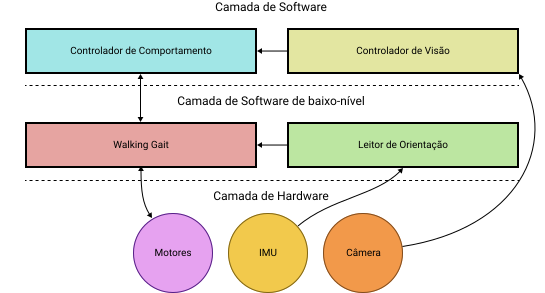
\includegraphics[scale=1]{imagens/svg/softwarearchitecture-flow}
	\caption{Visão simplificada da arquitetura do sistema e seus fluxos.}
	\label{fig:softwarearchitecture:overview}
\end{figure}

A figura~\ref{fig:softwarearchitecture:overview} mostra uma visão simplificada dos principais componentes -- e o sentido do fluxo de dados entre eles -- envolvidos no processo qualquer tarefa genérica. O funcionamento de cada componente individual será detalhado nas próximas seções.

\subsection{Visão}

Visão não é o foco deste trabalho. Entretanto, uma explanação geral é necessária afim de melhor entender o funcionamento geral do sistema.

\begin{figure}[h!]
	\centering
	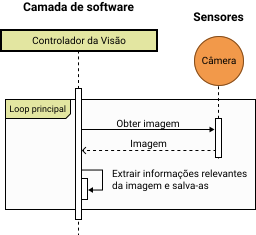
\includegraphics[scale=1]{imagens/svg/softwarearchitecture-vision}
	\caption{Diagrama de sequência do componente de visão.}
	\label{fig:softwarearchitecture:vision}
\end{figure}

O controle de visão é um software que conecta-se via USB com a câmera, analisando as imagens e extraindo informações relevantes à execução da tarefa do robô. De forma geral, podemos abstrair seu funcionamento em duas \textit{threads} distintas:

A primeira é o \textit{loop} principal, representada no diagrama de sequência na figura \ref{fig:softwarearchitecture:vision}. Em um primeiro passo, o controlador obtém a imagem da câmera. Em seguida, a extração de informações é realizada. Esse processo depende da tarefa que o robô deve realizar; tais como detectar a bola, os adversários e as linhas do campo, em caso de futebol ou detectar as linhas guia da pista de corrida no caso da maratona. Em seguida, tudo o que foi encontrado é salvo para futuras consultas até que a próxima iteração ocorra e os dados sejam atualizados.

A segunda \textit{thread}, visualizada na figura~\ref{fig:softwarearchitecture:software}, do controle de visão executa o sistema de comunicação que pode ser implementado de várias maneiras, desde objetos \textit{JSON} sendo transmitidos via \textit{UDP} até um \textit{message broker} com filas de consumo. Ao receber a mensagem de solicitação das informações, responde serializando os dados que ficaram salvos na primeira \textit{thread}, fornecendo as informações com atraso mínimo.

\subsection{Controlador de Comportamento}

O controlador de comportamento, que roda na camada de \textit{software}, implementa a tarefa que deve ser realizada pelo robô. Ele funciona como um gerente que coordena outros componentes, recebendo informações e enviando comandos com ações específicas serem a executadas. Na figura~\ref{fig:softwarearchitecture:software} é possível observar a sequência de passos realizados pelo controlador de comportamento.

Usando como exemplo uma partida de futebol, na figura~\ref{fig:softwarearchitecture:software} observa-se o controlador de comportamento ``jogador'' consultando o componente de visão, que responde a posição da bola, previamente obtida durante o processo da figura~\ref{fig:softwarearchitecture:vision}. Em seguida, baseado nessas informações o comportamento envia o comando ao \textit{walking gait} para caminhar na direção correta.

\begin{figure}[htb]
	\centering
	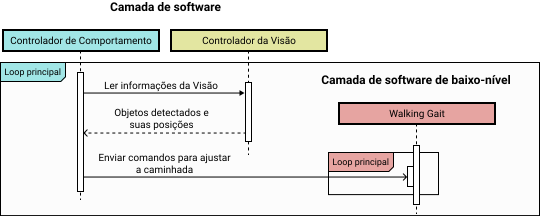
\includegraphics[scale=1]{imagens/svg/softwarearchitecture-software}
	\caption{Diagrama de sequência do controlador de comportamento e suas dependências.}
	\label{fig:softwarearchitecture:software}
\end{figure}

\subsection{\textit{Walking Gait} e Leitor de Orientação}

O componente \textit{walking gait} coordena e executa a caminhada. Ele monitora a USB aguardando os comandos de controle que contém as velocidades da caminhada, enviados a partir do controlador principal.

O componente leitor de orientação desempenha um papel importante ao lado do \textit{walking gait}. Ele é o responsável pela verificação da orientação da rotação do torso -- uma vez que a \textit{IMU} está situada nas costas de Arash -- assim fornecendo dados para o \textit{walking gait} fazer correções durante a caminhada afim de compensar um eventual distúrbio.

\begin{figure}[htb]
	\centering
	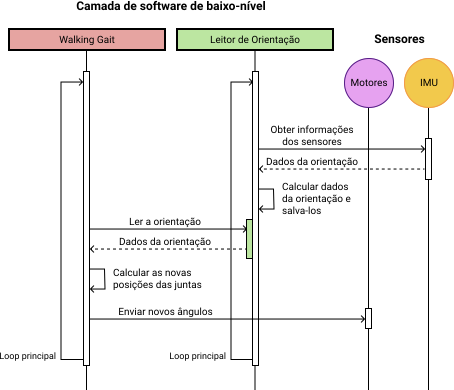
\includegraphics[scale=0.8]{imagens/svg/softwarearchitecture-lowlevel}
	\caption{Diagrama de sequência do \textit{walking gait} e do leitor de orientação.}
	\label{fig:softwarearchitecture:lowlevel}
\end{figure}

No componente leitor de orientação, os dados são coletados da \textit{IMU} e um processo de utilizando filtro de \todo{Explicar este processo melhor}\textit{Kalman} é utilizado para obter ua estimativa mais acurada das orientações que são salvas em variáveis. Já na \textit{thread} que roda o \textit{walking gait}, a orientação é continuamente consultada e utilizada para que os ângulos das juntas sejam atualizados.

Dentro da placa microcontroladora \textit{OpenCM9.04}, o \textit{walking gait} e o leitor de orientação rodam em \textit{threads} dinstintas, recurso este habilitado pela biblioteca \textit{MapleFreeRTOS}.

Na figura~\ref{fig:softwarearchitecture:lowlevel} observa-se a execução de ambas a \textit{threads} separadamente e a forma de interação entre elas. Iniciando a partir do \textit{walking gait}, ele lê os dados de orientação diretamente do leitor de orientação, em seguida calcula as posições das juntas que são enviadas aos motores. Em paralelo, o leitor de orientação continua recebendo os dados da \textit{IMU}, processando e salvando-os para que fiquem disponíveis ao \textit{walking gait}. Nota-se que, em ambas as threads, as sequências de ações são executadas dentro de \textit{loops} principais, já que este é um processo iterativo e contínuo.

\section{A nova arquitetura}

De acordo com os problemas e solução já discutidos em seções anteriores, esta seção irá apresentar as mudanças realizadas na arquitetura original apresentada na seção~\ref{sec:architecture:overview}.

Uma das principais mudanças realizadas neste trabalho é a re-implementação do \textit{walking gait}. Para tanto, ainda faz-se necessário a a utilização da \textit{OpenCM9.04}. Desta vez, ela assume o papel de reencaminhar os dados dos ângulos aos motores e, ainda, fornecer os dados de orientação ao \textit{walking gait}.

\begin{figure}[h!]
	\centering
	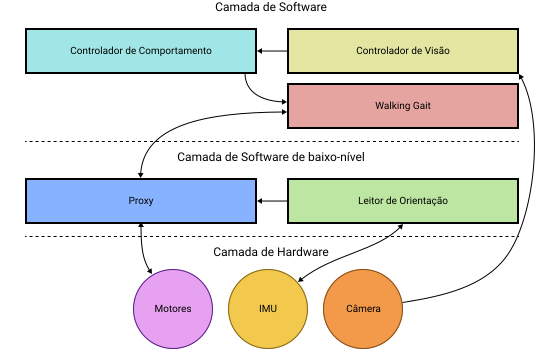
\includegraphics[scale=1]{imagens/svg/softwarearchitecture-newproposal}
	\caption{Diagrama de orientação dos atuadores de Arash.}
	\label{fig:softwarearchitecture:newproposal}
\end{figure}

A figura~\ref{fig:softwarearchitecture:newproposal} mostra a visão simplificada da nova arquitetura. Nela observa-se o \textit{walking gait} -- agora na camada de \textit{software} -- funcionando dentro do controlador principal, e um novo componente chamado \textit{proxy} é apresentado como interface os componentes de \textit{hardware} e o \textit{walking gait}. O papel do novo componente é de servir realmente como um \textit{proxy} enviando comandos recebidos do controlador principal aos motores e também receber a orientação do componente leitor de orientação e fornecê-la ao controlador principal.

O controlador de comportamento continua a enviar os comandos de controle ao \textit{walking gait}. Porém, ao invés de usar \todo{Especificar esses comandos na seção onde fala sobre esses comandos}comandos binários via \abrv[USB -- \textit{Universal Serial Bus}]{USB}, agora utiliza objetos serializados via \abrv[JSON -- \textit{Java Script Object Notation}]{JSON} via rede.

Entre o \textit{walking gait} e o \textit{proxy} a comunicação ocorre via USB @ 1 Mbps. Comandos de controle utilizando o \textit{dynamixel protocol 1.0} são gerados e enviados diretamente do \textit{walking gait} ao \textit{proxy}, que apenas os encaminha aos motores. Esta estratégia foi adotada para habilitar a possibilidade da utilização de motores de diferentes tipos, não apenas da Robotis Co. Assim, apenas o \textit{walking gait} é responsável pela geração de destes comandos específicos de cada motor enquanto o \textit{proxy} apenas os encaminha.

Na camada de software de baixo nível, o leitor de orientação continua a fornecer os dados de orientação. Porém, ao invés do \textit{walking gait} acessá-los diretamente, o \textit{proxy} encarrega-se de disponibiliza-los ao \textit{walking gait}.

\begin{figure}[h!]
	\centering
	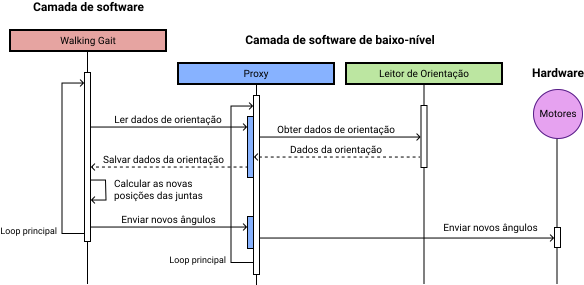
\includegraphics[scale=1]{imagens/svg/softwarearchitecture-newproposal-sequence}
	\caption{Diagrama de sequência simplificado com as modificações na arquitetura.}
	\label{fig:softwarearchitecture:newproposal:sequence}
\end{figure}

Na figura~\ref{fig:softwarearchitecture:newproposal:sequence}, é possível observar o diagrama de sequência com os componentes que foram atingidos pela mudança na arquitetura. O \textit{walking gait} lê os dados de orientação, calcula as novas posições das juntas e envia os novos ângulos ao \textit{proxy}, então inicia o processo do início. O \textit{proxy} obtém os dados de orientação diretamente do leitor de orientação, em seguida os fornece ao \textit{walking gait}.

\section{\textit{Walking gait}}

Nesta seção detalhes arquiteturais da implementação do \textit{walking gait} são descritos.

Ao realizar a nova implementação do \textit{walking gait}, uma mudança completa de paradigma foi realizada, do paradigma estruturado ao orientado a objetos. Afim de facilitar o desenvolvimento, o projeto foi divido em \todo{Conferir a quantidade de submódulo}$3$ submódulos: o servidor de controle, o motor de caminhada e o atualizador de juntas.

\subsection{Servidor de controle}

O servidor de controle é um submódulo que é habilita o \textit{walking gait} receber comandos de controle para saber a que direção deve caminhar.

Para realizar a tarefa de forma adequada, o componente faz uso de multi-processamento. Três \textit{threads} dentro do componente são responsáveis por tarefas específicas essenciais ao complemento do comportamento geral da caminhada: A \textit{thread} de rede, a \textit{thread} atualização dos motores e a \textit{thread} principal.

\subsection{\textit{Thread} principal: Da geração da trajetória até a aplicação às juntas}

\begin{figure}[h!]
	\centering
	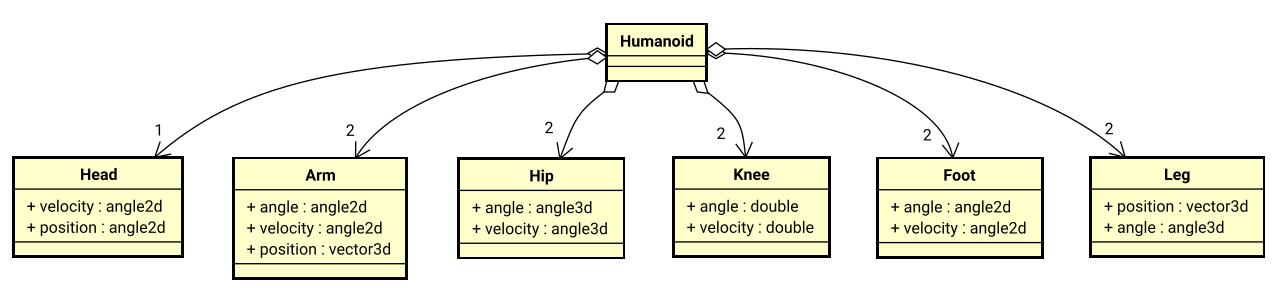
\includegraphics[scale=0.4]{imagens/svg/walkinggait-domain}
	\caption{Diagrama de domínio do \textit{walking gait}.}
	\label{fig:walkinggait:domain}
\end{figure}

A figura~\ref{fig:walkinggait:domain} mostra o diagrama de domínio das classes relevantes aos dados que o componente manipula. Nela podemos ver a classe $Humanoid$ é uma agregação de diversas outras classes que representam cada parte de Arash. É possível também observar que nas classes $Head$, $Arm$, $Hip$, $Knee$, $Foot$ existem dados ângulo e velocidade. Isso se dá por causa que componente utiliza essas informações para calcular o próximo estado do sistema em caso de algum distúrbio. Nota-se também, que a classe $Leg$ aparece de forma ambígua, já que existem as definições de $Hip$, $Knee$ e $Foot$. Porém, a classe $Leg$, representa os dados da cinemática inversa de uma perna, enquanto as demais classes guardam o estado atual das partes que representam.

Nota-se, também, a notação dos dados utilizados: $angle2d$, $angle3d$ e $vector3d$. Note que todos os tipos possuem o sufixo numérico, que indica a quantidade de dimensões aquela classe guarda, e a letra, que indica o tipo de seus dados, no caso $d$ que significa $double$. Para ângulos, $2$ dimensões significa que as dimensões $pitch$ e $roll$ são guardadas; já para $3$ dimensões as orientações $roll$, $pitch$ e $yaw$ são guardadas. Para vetores, os valores $x$, $y$ e $z$ são guardados.

\subsection{Abstração dos motores}
\label{subsec:motors_abstraction}